% This is samplepaper.tex, a sample chapter demonstrating the
% LLNCS macro package for Springer Computer Science proceedings;
% Version 2.20 of 2017/10/04
%
\documentclass[runningheads]{llncs}
%
\usepackage{graphicx}
\usepackage{hyperref}
% Used for displaying a sample figure. If possible, figure files should
% be included in EPS format.
%
% If you use the hyperref package, please uncomment the following line
% to display URLs in blue roman font according to Springer's eBook style:
% \renewcommand\UrlFont{\color{blue}\rmfamily}

\begin{document}

\title{SPANG Template Library: Making SPARQL Queries FAIR}
\titlerunning{SPANG: Making SPARQL Queries FAIR}
\author{Hirokazu Chiba}
\authorrunning{H. Chiba}
\institute{Database Center for Life Science, Chiba 277-0871, Japan\\
\email{chiba@dbcls.rois.ac.jp}
}
%
\maketitle              % typeset the header of the contribution
%
\begin{abstract}
%The abstract should briefly summarize the contents of the paper in 15--250 words.
How can we maximize the value of accumulated SPARQL queries? 
%SPARQL is a key component of the Semantic Web, thus the reusability of SPARQL is important.
An increasing number of datasets have been published in the Resource Description Framework (RDF) and the SPARQL standard allows interoperable framework for querying the RDF datasets; however, reuse of SPARQL queries remains limited partly due to the lack of accessibility and findability of SPARQL queries that were once written. 
%SPARQL contributes to the standardized interface to the RDF, and maximizing the reusability of RDF; however, reusability of SPARQL itself remains to be addressed. 
In this study, we focus on FAIR (findable, accessible, interoperable,
reusable) principle to improve usability of SPARQL queries.
We present the process of making SPARQL queries FAIR and demonstrate the usefulness of the result.
FAIRification of the SPARQL is a plausible way to make SPARQL interoperable and reusable.
Here, we define a SPANG library as a controleld query set with specific
extension of SPARQL so that the query set follows FAIR pinciple.
%Here we propose a SPARQL extension to construct a reusable query library to enrich the Semantic Web platform.
Our contribution is the improvement of findability and accessibility of SPARQL queries.
1) We present a metadata set for annotating a SPARQL query, which
enables to identify SPARQL query and provides useful information for the query.
2) We present a mechanism to parameterize the SPARQL query.
It makes each query reusable in different settings.
This study make SPARQL queries FAIR, and this specification leads to the construction of eco-system to reuse SPARQL queries to enrich the use of the Semantic Web platform.

\keywords{SPARQL \and FAIR \and query library}

\end{abstract}


%%%%%%%%%%%%%%%%%%%%%%
\section{Introduction}
%%%%%%%%%%%%%%%%%%%%%%

How can we maximize the value of accumulated SPARQL queries?
Reuse of them is the key.
An increasing number of datasets have been published in the Resource Description Framework (RDF).
SPARQL is the standardized interface to RDF and contributing the reusability of the RDF data. 
Although the SPARQL language provides a basis for exploiting RDF databases, writing a raw SPARQL code often becomes a burden for users. 
SPARQL is the standardized query language, and many Semantic Web users write queries in SPARQL, with a great amount of efforts.
Those queries are valuable resource.
Reusability is the key to maximize the value of accumulated open data and software.
However, due to the limitation of SPARQL specifications, the reuse of those queries are limited. 
Reusing SPARQL queries are important for efficient development of the Semantic Web.

The FAIR principle~\cite{fair} could be suitable for addressing this issue.
One of the key principle in recent days of the Semantic Web community is the FAIR principle: findable, accessible, interoperable and reusable.
As the SPARQL queries are important component of the Semantic Web community,
they should be shared in a solid principle.
The Semantic Web is comprised of various specifications, including RDF~\cite{rdf}, OWL~\cite{owl}, and SPARQL~\cite{sparql}. The ontologies written in OWL are accumulated and shared on repositories~\cite{bioportal}.
RDF datasets are also accumulated and hosted in portal web sites~\cite{rdf-portal}.
Not only the ontologies and datasets, but also the queries are important for the Semantic Web.
Accumulating and reusing the queries are important.
Interestingly, the FAIR principle can be applied not only to the RDF data, but also other resource, like software.
SPARQL is a fundamental technology for querying RDF data contributing an interoperable interface to the Semantic Web. However, is is not designed for reusability. 
In data management guideline, FAIR principle is well known~\cite{fair}. Findability, Accesibility, Reusablility should be addressed, to make the most of SPARQL queries as resources. 

%How can we make SPARQL queries fair? 
Are SPARQL queries accessible? In most cases, those queries are not accessible. According to the FAIR principle, resources should be accessible by through URI. In some cases, SPARQL queries are stored in repositories. But they do not have stable URIs. How about findability? In many Semantic Web projects, SPARQL queries are written and accumulated. However, those SPARQL queries are not findable, due to the lack of export and import SPARQL queries.

Here, we decided to follow the FAIR principle and extend the SPARQL specifications for more efficient development of the Semantic Web.
Semantic Web users often write SPARQL queris.
However, the SPARQL lacks the parameterization mechanism, thus, users write queries for their specific use cases.
But good SPARQL queries can be reused.
Actually, writing good query requires much efforts, thus, they should be reused to improve the productivity.
Thus, considering the reusability of SPARQL queries are crucial to enrich the Semantic Web community.
How can we improve the reusability of SPARQL?
One of the key to improve the reusability of queries is parameterization.
Parameterization make the query more reusable.
Using the template query with parameters, the same query can be applied to many use cases.
% There can be several types of parameterization.
% The SPARQL variables can be considered as parameter.
% In that case, values to the parameters can replace them.
% On the other hands, part of the URI or literals can be parameterized.
% In that case also, values to the parameters can replace them.
% Another mechanism to use template is to give binding to the variables.

Contributions of this work is 
1) we provide a SPARQL meta data required for constucting SPARQL queries;
2) we constructed template engines for SPARQL queries; and
3) we constructed controlled SPARQL queries for available SPARQL endpoints.




%%%%%%%%%%%%%%%%%%%%%%%%
\section{Overview}
%%%%%%%%%%%%%%%%%%%%%%%%

We overview the FAIR principles, then describe how to apply the principle to SPARQL.
We demonstarate how to use the SPANG templete library.
Then, we describe the details of SPANG template specifications.

%The following section includes: overview of the SPANG project, specification of SPANG templates, implementation of the SPANG library, and use case of SPANSG library.

Figure~\ref{fig:spang_top} is the top page of SPANG, which includes links to GitHub, Documentation, and SPANG library.

\begin{figure}
\center
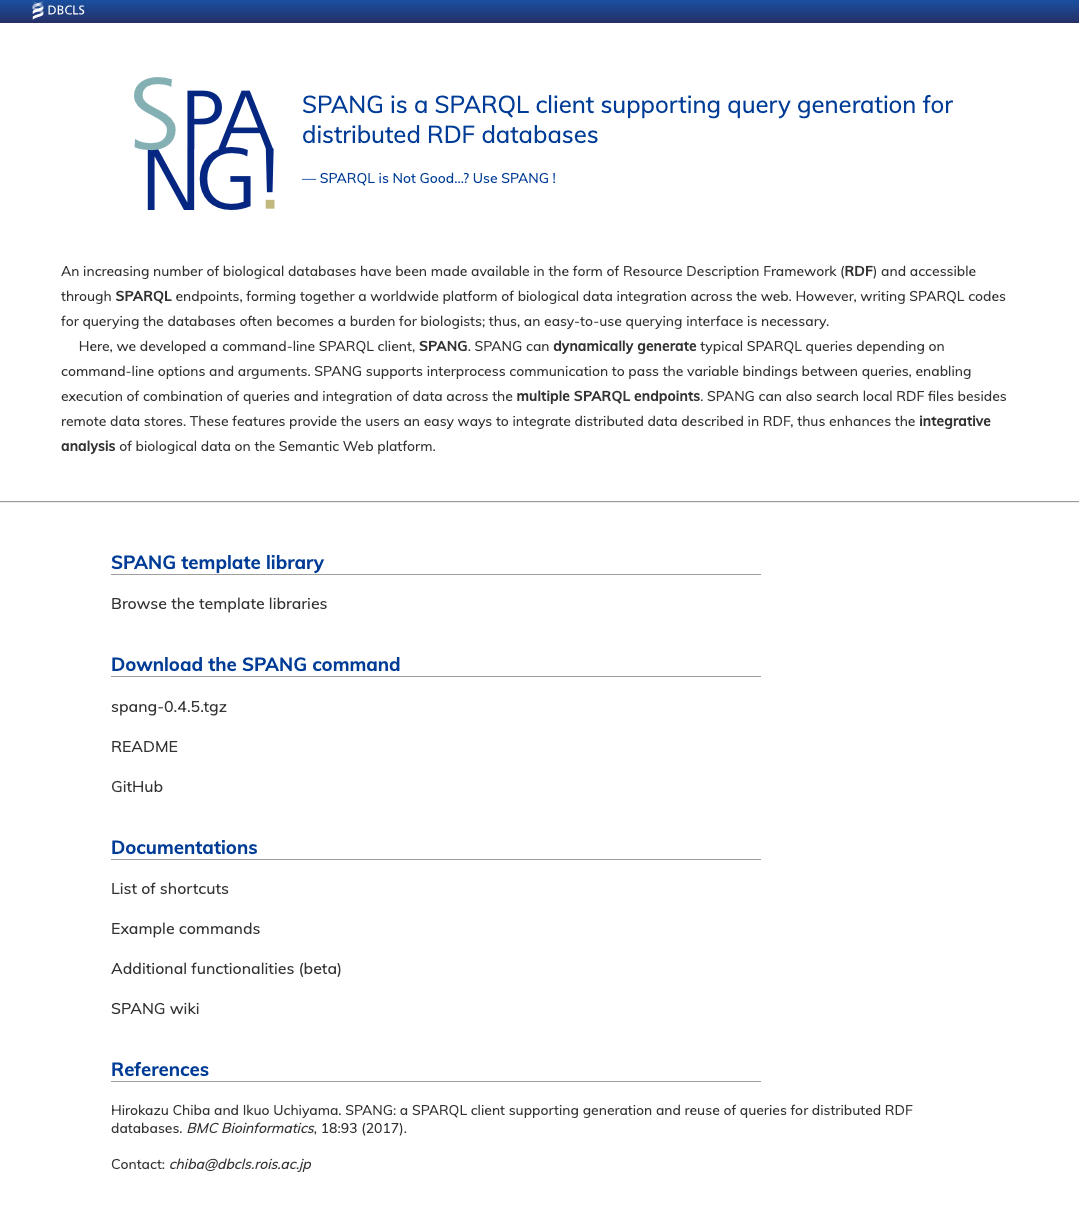
\includegraphics[width=1.0\textwidth]{spang_top.png}
\caption{SPANG server top page}
\label{fig:spang_top}
\end{figure}


%%%%%%%%%%%%%%%%%%%%%%%%
\section{Making SPARQL Queries FAIR}
%%%%%%%%%%%%%%%%%%%%%%%%

The FAIR guiding principle aims to enhance the Findability, Accessibility, Interoperability and Reusability of digital resources.

Not only the RDF dataset, but also the SPARQL queries are important resource to be shared on the Semantic Web platform. Thus, we applied the FAIR principle which have been applied to the RDF datasets, into SPARQL queries.

Here we overview the preliminaries for the FAIR principle.
It shoulbe noted that the FIAR principle can be applied not only to the dataset resources but also to other type of resources including software tools.

Here, we provide the FAIR principle in the context of SPARQL queries.


In the previous section, we showed the core idea of the FAIR principle.

So, what is the relationship between FAIR principle and the Semantic Web?
The core technology constituting the Semantic Web is RDF, OWL, and SPARQL. RDF and OWL follows the FAIR principle. However, SPARQL is not FAIR.

So, what is the problem of the FAIRification status of SPARQL?
SPARQL is important component of the Semantic Web. The use of SPARQL query is essential for the Semantic Web community.

The key is the metadata.

Here, we constructed SPANG library: a SPARQL library which is findable, accessible, interoperable and reusable.

The process of making SPARQL FAIR ("FAIRification") can be described in multiple steps~\cite{fairification}.
Most of the requirements for findability and accessibility can be achieved at the metadata level. Interoperability and reuse requires more efforts at the SPARQL code level.


\subsection{Findability}
The first step is using data to find SPARQL queries. Metadata should be easy to find for both humans and computers. Machine-readable metadata are essential for automatic discovery of resources, so this is essential component.
% \begin{itemize}
%     \item Assign global identifier
%     \item Rich metadata
%     \item Include the identifier of the data they describe
%     \item Registered and indexed
% \end{itemize}

Most of the SPARQL queries are not findable from general users of the Semantic Web. The first and most important step toward increased value of the written SPARQL queries is to consider how to make SPARQL queries findable.
In the FAIR principle, making resources findable includes indexing resources by adding metadata to each resources. 
To make SPARQL queries findable, we propose to add metadata to SPARQL.
The SPARQL metadata includes: title, description, target endpoint, and parameters with its name, default value, and classes.

Indexing of SPARQL queries are conducted and thus users can obtain specific queries of interest through a search API.

\subsection{Accessibility}
Once the user finds the required data, the user needs to know how can they be accessed, possibly including authentication and authorisation.
% \begin{itemize}
%     \item Retrievable by identifier
%     \item Metadata are accessible
% \end{itemize}

Some of the SPARQL libraries are accessible from internet. Howver, we could consider more general scheme for accesibility. In the FAIR principle, accessibility includes minting URI for each resource. Here we propose to use stable URI for each SPARQL query.
In the case of SPANG library, we assign two URI for each query. One is for retrieving SPARQL query string, thereby users can retrieve the concrete content of the query. Another is URI to get results. This URI can include the parameter settings for the specified query.

\subsection{Interoperability}
The ultimate goal of FAIR is to optimise the reuse of data. To achieve this, metadata should be well-described so that they can be replicated and/or combined in different settings.
% \begin{itemize}
%     \item Richly described with a plurality of accurate and relevant attributes
%     \begin{itemize}
%         \item released with a clear and accessible data usage license
%         \item associated with detailed provenance
%         \item meet domain-relevant community standards
%     \end{itemize}
% \end{itemize}

The data usually need to be integrated with other data. In addition, the data need to interoperate with application or workflows for analysis, storage, and processing.
% \begin{itemize}
%     \item Use a formal, accessible, shared, and broadly applicable language for knowledge representation.
%     \item Use vocabularies that follow FAIR principles.
%     \item Include qualified references to others
% \end{itemize}

SPARQL specification is proposed for interoperable use of queries to the Semantic Web. It is valuable to use several triplestore implementation through the same programming interface. However, no rule is proposed for coding rules; capitalization, indentation and newline, etc. Lack of those rules result in variation of SPARQL queries, which hampers the reuse of SPARQL queries. In other languages, some coding ruels exist. In the case of SPARQL, specification document or text books do not follow a specific coding rules. Here, we specify the coding rule used in SPANG template library, and implemented spfmt command to reformat of the code.

\subsection{Reusability}
Reusability of SPARQL is not a new topic. Various activity is conducted to construct libraries of SPARQL. It is considered as acitivities to increase the reusability of SPARQL queries. However, no standard to increase the reusability is proposed. In the specifiation of SPARQL, reusability is not a centroal topic. However, it is an central resource in a Semantic Web. If it is a component of Semantic Web comprised of RDF/OWL/SPARQL, it is reasonable to represent it in RDF framework. We propose a way to represent SPARQL in the RDF framework.

Templating is also a key issue for reusability. SPARQL specifications do not includes templating mechanism, but without templating, each SPARQL queries are not applicable to other use cases. We implemented templating mechanism using a general freamework, mustash.




\begin{figure}[!t]
\begin{scriptsize}
\begin{verbatim}
# @title Get UniProt IDs for a specific disease, e.g. C0751955 ("Brain Infarction")
# @endpoint http://rdf.disgenet.org/sparql/
# @prefix https://raw.githubusercontent.com/hchiba1/spang-library/master/prefix/bio
# @param arg1=C0751955 

PREFIX disgenet_source: <http://rdf.disgenet.org/v4.0.0/void/>
PREFIX umls: <http://linkedlifedata.com/resource/umls/id/>

SELECT DISTINCT ?gene ?score ?gene_label ?source ?gda ?pmid ?description
WHERE {
    ?gda sio:SIO_000628 umls:{{arg1}} ,
                        ?gene ;
          a ?type ;
          sio:SIO_000253 ?source ;
          sio:SIO_000216/sio:SIO_000300 ?score .
    ?gene a ncit:C16612 ;
          rdfs:label ?gene_label .
    OPTIONAL {
        ?gda sio:SIO_000772 ?pmid ;
             dct:description ?description .
    }
}
ORDER BY DESC(?score) ?source ?pmid

\end{verbatim}
\end{scriptsize}
\caption{Example query in SPANG library}
\label{fig:example-rdf}
\end{figure}

%%%%%%%%%%%%%%%%%%%%%%%%%
\section{SPANG Library and Use Cases}
%%%%%%%%%%%%%%%%%%%%%%%%%

The core of the SPANG specification is the SPARQL metadata and templating mechanism for increasing the reusability of the SPARQL queries.

An example query in the SPANG library is shown below.
The DisGeNet endpoint~\cite{disgenet} is specified.


\subsection{SPARQL Metadata}

We propose a set of SPARQL metadata to annotate each SPARQL query, to make them more reusable.
Those metadata are added as comment at the head of the SPARQL query, thus that does not violate the SPARQL specification. 
The set of metadata increase the findability of SPARQL queries.

As a use case, we developed a SPANG API to search for the set of SPARQL queries.

\subsection{SPARQL Parameterization}

We propose the parapeterization mechanism of SPARQL query. It is crucial to reuse the SPARQL query for us to improve the productivity of the programming experiance on the Semantic Web platform.

Using SPANG API, users can execute SPARQL query over the Web, with the given parameters.


\subsection{SPANG Library API}
According to the metadata and parameterization mechanism, we can construct a controlled set of SPARQL library which is reusable in various settings.

SPANG library is accesible through SPANG Web API.

The following command returns the list of libraries.

\texttt{curl https://spang-portal.dbcls.jp/api/library}

The results is shown in Figure~\ref{fig:libs-api-out} as JSON format.


The following command returns the list of query in a library.

\texttt{curl https://spang-portal.dbcls.jp/api/library/disgenet}

The results is shown in Figure~\ref{fig:lib-api-out} as JSON format.

\subsection{SPANG Query API}

The following command returns the result of the query, with the given paramter.

\texttt{curl https://spang-portal.dbcls.jp/api/library/disgenet/gene\_disease.rq?arg1=678}



Figure~\ref{fig:spang_disease_gene_query} shows a query for DiesGeNet SPARQL endpoint to get disase gene relationship. 
Figure~\ref{fig:spang_disease_gene_result} shows the result of the query. Thus, users can get the results only by clicking on the web pages, browsing the SPARQL template on the SPANG web site.


The following command searches for queries with keywords.


\subsection{SPANG Server}
SPANG is originally developed for "SARQLing" the RDF dataset from command line. Here, we re-implemented the SPANG using Node.js and now the functionality is available through Web browser. 


Figure~\ref{fig:spang_lib} is the list of the target SPARQL endpoints. It also lists the SPARQL templates available in general for various endpoints.

Figure~\ref{fig:spang_lib} is the list of SPARQL templates for DisGeNet SPARQL endpoint.
A short name for the SPARQL template, descriptin of the query, and example parameters are shown.


\begin{figure}
\center
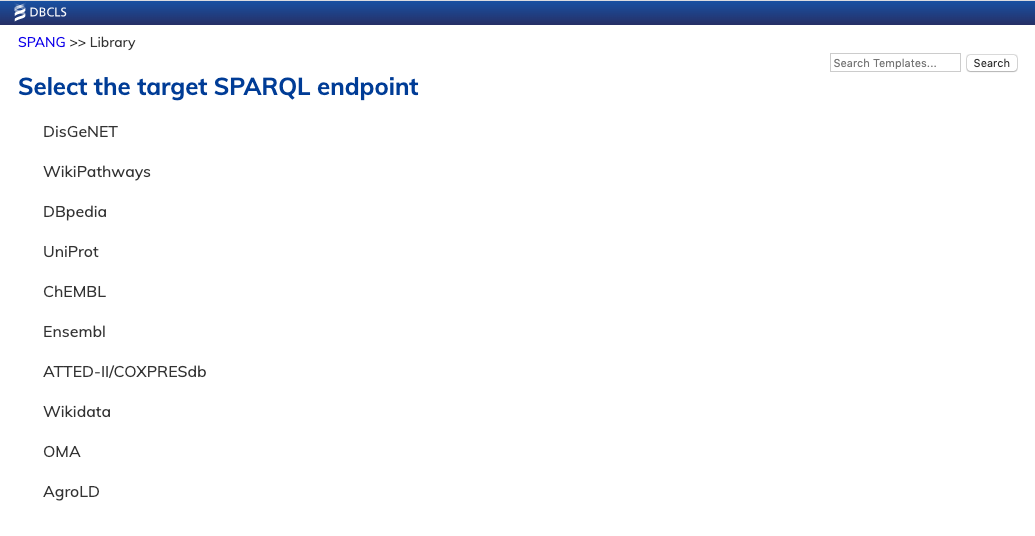
\includegraphics[width=1.0\textwidth]{spang_lib.png}
\caption{SPANG library}
\label{fig:spang_lib}
\end{figure}


\begin{figure}[!t]
\begin{scriptsize}
\begin{verbatim}
[
  {
    "name": "disgenet",
    "title": "DisGeNET",
    "description": "DisGeNET",
    "endpoint": "http://rdf.disgenet.org/sparql/",
    "schema": "http://www.disgenet.org/web/DisGeNET/menu/rdf#schema",
    "uri": "http://localhost:7070/api/library/disgenet",
    "count": 14
  },
  {
    "name": "wikipathways",
    "title": "WikiPathways",
    "description": "WikiPathways",
    "endpoint": "http://sparql.wikipathways.org/",
    "schema": null,
    "uri": "http://localhost:7070/api/library/wikipathways",
    "count": 6
  },
  ...
]
\end{verbatim}
\end{scriptsize}
\caption{List of in query libraries obtained by API}
\label{fig:libs-api-out}
\end{figure}


\begin{figure}
\center
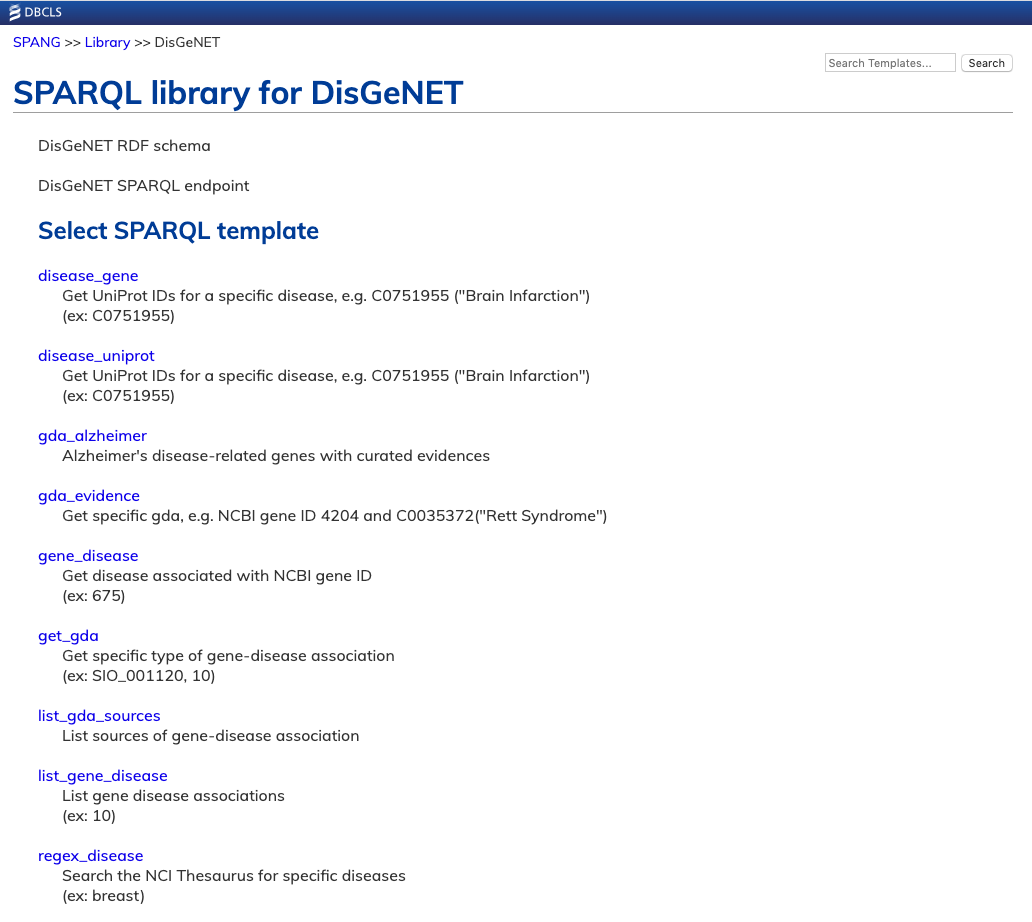
\includegraphics[width=1.0\textwidth]{spang_disgenet.png}
\caption{SPANG templates for DisGeNet SPARQL endpoint}
\label{fig:spang_disgenet}
\end{figure}



\begin{figure}[!t]
\begin{scriptsize}
\begin{verbatim}

{
  "disgenet": [
    {
      "name": "disease_gene",
      "title": "Get UniProt IDs for a specific disease, e.g. C0751955 (\"Brain Infarction\")",
      "uri": "http://localhost:7070/api/disgenet/disease_gene",
      "endpoint": "http://rdf.disgenet.org/sparql/",
      "param": [
        {
          "name": "arg1",
          "default": "C0751955"
        }
      ]
    },
    {
      "name": "disease_uniprot",
      "title": "Get UniProt IDs for a specific disease, e.g. C0751955 (\"Brain Infarction\")",
      "uri": "http://localhost:7070/api/disgenet/disease_uniprot",
      "endpoint": "http://rdf.disgenet.org/sparql/",
      "param": [
        {
          "name": "arg1",
          "default": "C0751955"
        }
      ]
    },
    {
      "name": "gda_alzheimer",
      "title": "Alzheimer's disease-related genes with curated evidences",
      "uri": "http://localhost:7070/api/disgenet/gda_alzheimer",
      "endpoint": "http://rdf.disgenet.org/sparql/",
      "param": [

      ]
    },
    {
      "name": "gda_evidence",
      "title": "Get specific gda, e.g. NCBI gene ID 4204 and C0035372(\"Rett Syndrome\")",
      "uri": "http://localhost:7070/api/disgenet/gda_evidence",
      "endpoint": "http://rdf.disgenet.org/sparql/",
      "param": [

      ]
    },
    ...
  ]
}

\end{verbatim}
\end{scriptsize}
\caption{Search results obtained by API}
\label{fig:lib-api-out}
\end{figure}


\begin{figure}
\center
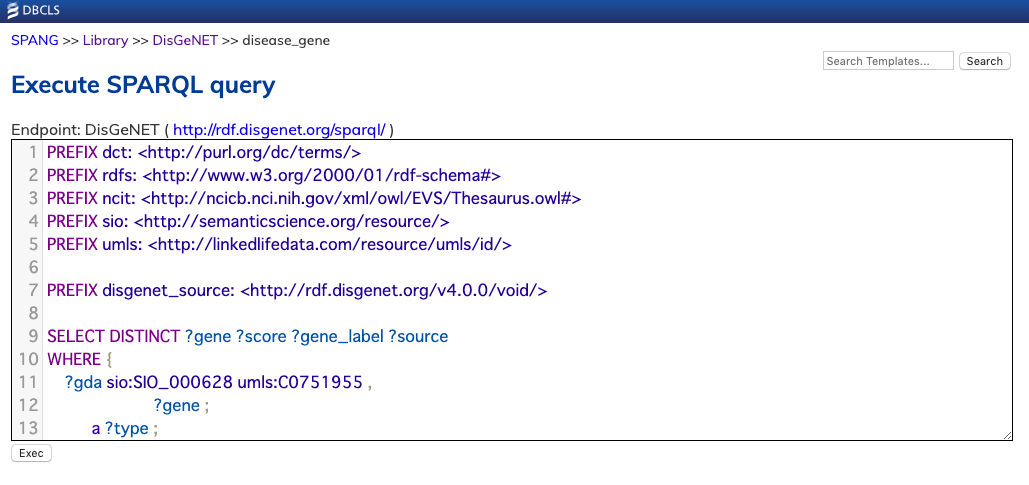
\includegraphics[width=1.0\textwidth]{spang_disease_gene_query.png}
\caption{SPANG templates for DisGeNet SPARQL endpoint}
\label{fig:spang_disease_gene_query}
\end{figure}

\begin{figure}
\center
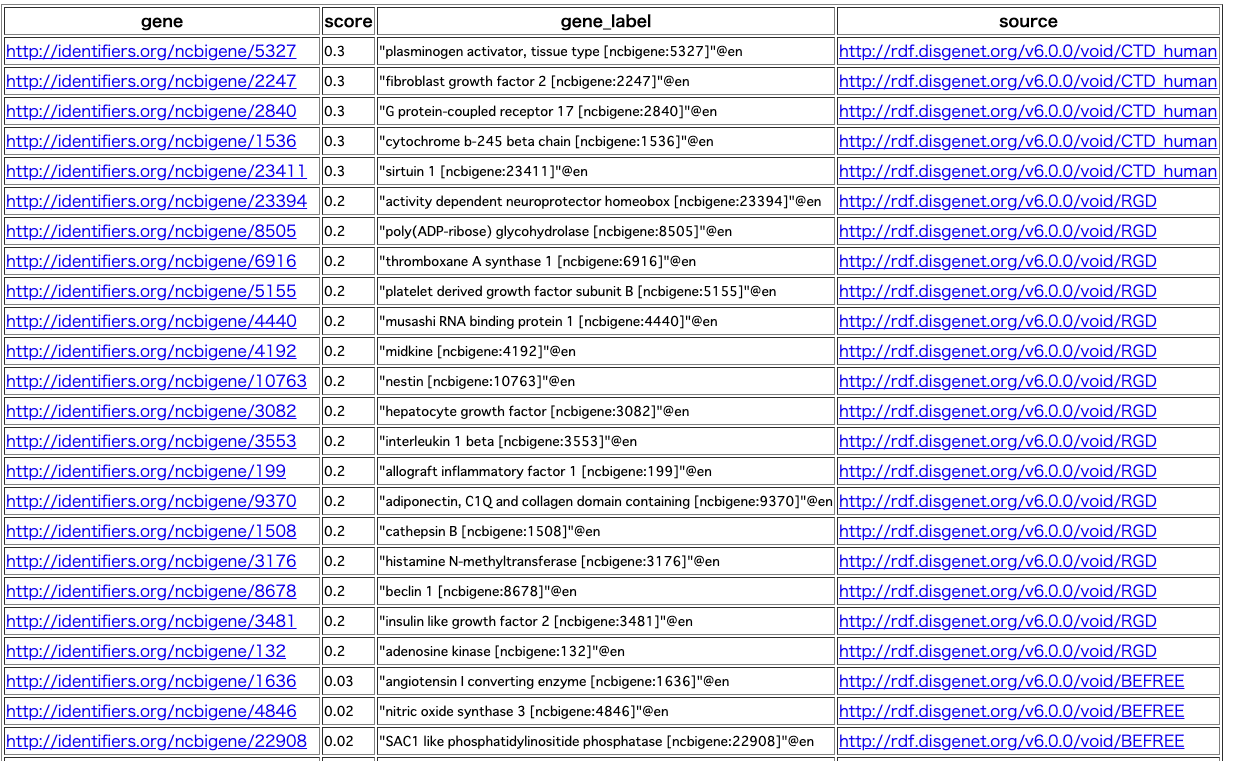
\includegraphics[width=1.0\textwidth]{spang_disease_gene_result.png}
\caption{SPANG templates for DisGeNet SPARQL endpoint}
\label{fig:spang_disease_gene_result}
\end{figure}




\texttt{curl https://spang-portal.dbcls.jp/api/search?keyword=gene}


%%%%%%%%%%%%%%%%%%%%%%%%%
\section{Specifications}
%%%%%%%%%%%%%%%%%%%%%%%%%

SPANG is implemented in JavaScript using the Node.js technology~\cite{nodejs}. Thus, it can be called in JavaScript applications, and also in the command-line environment.

\subsection{Template Specifications}
SPANG template syntax is an extension of sparql-doc. Although the sparql-doc aims at documentation of SPARQL originally, this notation is suitable for annotating each SPARQL query with metadata in the frame of SPARQL query. Each query can be still used as standard SPARQL query, and furthermore, if a parser for comment liens is implemented, users can obtain the metadata for the queries.
Here, we consider the parameterization in this frame. We consider the parameters of the query as metadata of SPARQL.
As a syntax parameterization, we consider mustash notation.


\subsection{Template Engine}
SPANG template engine is implemented, where each template can be transformed into abstract syntax tree, and then reconstructed into SPARQL. 
We used PEG~\cite{peg} expression of SPARQL grammar originally expressed in EBNF in the SPARQL specification. The original implementation of PEG.js~\cite{pegjs} of SPARQL grammar is provided by rdfstore-js project (https://github.com/antoniogarrote/rdfstore-js).
The PEG.js code was modified to fit the use in the case of SPANG library.
The PEG.js is a parser generator, thus, we could generate our own parser based on the PEG.js description. Thus, we obtained abstract syntax tree in the form of JSON object.

We also developed a formatter to stringify the JSON object into string text. Thus, we can reformat the input SPARQL.


\subsection{Coding Rules}
We defined a coding rule for SPARQL and its extension in SPANG framework. Coding rule is important for productivity of shared coding tasks and effective maintenance. It also helps to make debug process easier; weird look suggests possible bugs. 
\begin{itemize}
    \item Header lines: query can start with header lines as comment lines. Metadata can be added at the top of the query as comment lines. Multiple lines are allowed. If multiple lines are described, they are written in sequential without blank lines. After the metadata lines, a blank line comes.
    \item Prefix: prefix declaration comes in sequential lines. Each of before and after the prefix declaration lines, a blank line exists.
    \item Cases: the SPARQL keywords should be in upper case characters. variable names comes with ? followed by lower case characters.
    \item Literal: the literals are surrounded by "".
    \item Indent: indentation depth is two spaces.
    \item Spaces: a space exists between keywords and variables. A space exists before , or ; or . .
    \item Newline: a newline exists before the keyword \texttt{WHERE} and after \texttt{\{}. A new line exist after ; or . but not after ,. After the newline following ;, an indent follows. A newline exist before query modifiers such as \texttt{ORDER BY} or \texttt{LIMIT}.
\end{itemize}
We developed a reformatter of the SPARQL code as described below.


%%%%%%%%%%%%%%%%%%%%%%
\section{Availability}
%%%%%%%%%%%%%%%%%%%%%%


\subsection{JavaScript Application}
SPANG is now implemented in JavaScript, so the SPARQL queries can be executed in JavaScript code across the internet. To avid CORS retriction, it can access through content delivery network services, such as jsDelivr~\cite{jsdelivr}, as shown in Figure~\ref{fig:jsdelivr}.



\begin{figure}[!t]
\begin{scriptsize}
\begin{verbatim}
spang.getTemplate('https://cdn.jsdelivr.net/gh/hchiba1/spang-library@latest/library/uniprot/count_org.rq', 
(template) => {
  result = spang.query(template, 'https://sparql.uniprot.org', { abbr: true, format:'tsv'}, 
  (error, res, body) => { console.log(body); });
});
\end{verbatim}
\end{scriptsize}
\caption{Use of SPARQL library in a JavaScript application}
\label{fig:jsdelivr}
\end{figure}


\subsection{Command-line Client}
As an interface the the SPANG library, we constructed a command-line interface.
Originally, SPANG was developed as a command line client in Perl~\cite{spang}.
It is re-implemented in JavaScript using Node.js as \texttt{SPANG2}.
SPARQL templates can be executed in command line.
The following example command line gives a parameter to the query template, and execute to the DisGeNet endpoint

\texttt{spang2 disease\_gene.rq --param disease=C0751955}

The template can be URL that returns a SPARQL query, such as \url{https://cdn.jsdelivr.net/gh/hchiba1/spang-library@latest/library/disgenet/disease_gene.rq}. The full usages of the command is as shown in Figure~\ref{fig:spang-command}.


\begin{figure}[!t]
\begin{scriptsize}
\begin{verbatim}
Usage: spang2 [options] <SPARQL_TEMPLATE>

Options:
  -e, --endpoint <ENDPOINT>    target SPARQL endpoint
  -p, --param <PARAMS>         parameters to be embedded (in the form of "--param par1=val1,par2=val2,...")
  -o, --outfmt <FORMAT>        tsv, json, n-triples (nt), turtle (ttl), rdf/xml (rdfxml), n3, xml, html
  -a, --abbr                   abbreviate results using predefined prefixes
  -v, --vars                   variable names are included in output (in the case of tsv format)
  -S, --subject <SUBJECT>      shortcut to specify subject
  -P, --predicate <PREDICATE>  shortcut to specify predicate
  -O, --object <OBJECT>        shortcut to specify object
  -L, --limit <LIMIT>          LIMIT output (use alone or with -[SPOF])
  -F, --from <FROM>            shortcut to search FROM specific graph (use alone or with -[SPOLN])
  -N, --number                 shortcut to COUNT results (use alone or with -[SPO])
  -G, --graph                  shortcut to search for graph names (use alone or with -[SPO])
  -r, --prefix <PREFIX_FILES>  read prefix declarations (default: SPANG_DIR/etc/prefix,~/.spang/prefix)
  -n, --ignore                 ignore user-specific file (~/.spang/prefix) for test purpose
  -m, --method <METHOD>        GET or POST (default: "GET")
  -q, --show_query             show query and quit
  -f, --fmt                    format the query
  -i, --indent <DEPTH>         indent depth; use with --fmt (default: 2)
  -l, --list_nick_name         list up available nicknames of endpoints and quit
  -d, --debug                  debug (output query embedded in URL, or output AST with --fmt)
  -V, --version                output the version number
  -h, --help                   output usage information

\end{verbatim}
\end{scriptsize}
\caption{Usage of the \texttt{SPANG2} command}
\label{fig:spang-command}
\end{figure}


\subsection{SPANG Server}
SPARQL queries can be executed in Web site.
SPANG server is developed using Ruby on Rails. And it can be run on Docker. The SPANG query library is published on GitHub. Thus, users can run a portal site by their own. The SPANG APIs are available on the SPANG server.


% \subsubsection{Calling libraries}

% Although SPARQL shortcuts are useful for simple querying with typical query patterns, they do not cover various
% queries with complicated patterns. 
% Thus, SPANG provides a mechanism to accept SPARQL templates to generate arbitrary query patterns. 
% An example query is: 

% \texttt{spang uniprot taxtree\_ancestor 511145 -ac}

% \noindent where the first argument is the target SPARQL endpoint and the following arguments are SPARQL templates and parameters. {\tt taxtree\_ancestor} is the name of a SPARQL template included in the predefined SPARQL library (see supplementary data for the code), {\tt 511145} is the parameter, {\tt -a} is the option for abbreviating results, and {\tt -c} is for aligning output columns for easier reading.
% The specified parameter replaces the placeholder included in the template before execution. 
% This example query traverses the NCBI taxonomy tree from the given ID (511145) to the root node and outputs scientific names in each taxonomic rank.


% Available SPARQL templates are not limited to the local library.
% If SPARQL libraries are published on the Web, the users can call the templates by means of URIs across the Web.
% An example usage of the Microbial Genome Database (MBGD) SPARQL library published at http://mbgd.genome.ad.jp/sparql/library/ is as follows.

% \texttt{spang mbgd mbgdl:get\_ortholog K9Z723}

% where {\tt mbgd} is the MBGD SPARQL endpoint \citep{Chiba} and \texttt{mbgdl:} is a prefix for abbreviating the URI of the template {\tt get\_ortholog} in the MBGD SPARQL library (see supplementary data for the code). 
% The template can be specified in the full URI or in abbreviated form using the predefined prefix declarations.
% This example query searches the MBGD database \citep{Uchiyama} for the orthologs of a protein \texttt{K9Z723} (Photosystem II lipoprotein Psb27).


% \subsubsection{Combinatorial execution}

% SPANG combines multiple queries through a Unix pipe. 
% Combining a {\tt spang} command in shortcut mode and another one in template mode is also possible.
% An example of such a combinatorial query is shown in Fig.~\ref{fig:01}.
% The first {\tt spang} command is in template mode, which is the same as that presented in the Section 2.3. 
% This command searches the MBGD database for orthologs of a protein {\tt K9Z723}. 
% The obtained list of proteins are used in the second query, which searches the UniProt database for annotations of the given list of proteins. 
% The option \texttt{-S 1} specifies the values from the first column of the standard input as subject.
% This combinatorial query enables integrative use of two databases distributed across the Web. 
% Here, the output of the first command can be further modified by altering the second command.
% For example:
% \begin{quoting}
% \texttt{spang mbgd mbgdl:get\_ortholog K9Z723 | spang uniprot uniprot\_xref PDB}
% \vspace{1pt}
% \end{quoting}
% where {\tt uniprot\_xref} is a SPARQL template (see supplementary data for the code), which retrieves cross-references from the UniProt IDs given in the standard input to the database specified as the parameter (in this example, {\tt PDB}). This example command line searches for entries in the Protein Data Bank (PDB) \citep{Berman} among orthologs of {\tt K9Z723}.



%%%%%%%%%%%%%%%%%%%%%%
\section{Related Work}
%%%%%%%%%%%%%%%%%%%%%%

SPARQL tempalting mechanisms have been implemented in various projects. Based on the templating mechanisms, SPARQL libraries have been implemented, such as Bioqueries. SPARQList is a framework to store SPARQL templates to be used through API.

As a SPARQL formatter, some software are available.
rdfstore-js\cite{rdfstore-js} has SPARQL parser, but does not have formatter.
SPARQL.js~\cite{sparql-js} implements parser and formatter. However, there are no formatting rule explicitly defined.
Jena package~\cite{jena} includes parser and formatter. However, it does not define formatting rule.

Bioqueries~\cite{bioqueries} have tried to collect SPARQL queries as community effort. It increase the findability and reusability.
However, the query can only be executed on the web site.
Users should copy and paste the queries into their own software.
In contrast, we tried to build a software network on top of the Semantic Web platform.

SPARQList~\cite{sparqlist} is a REST API server which executes a SPARQL query, transform the result into formatted data if defined. In SPARQList, configuration of the SPARQL queries such as parameters of the API, SPARQL endpoints is written in the Markdown format. SPARQList server can be considered as a repository of SPARQL queries. In terms of the FAIR principle, findability should be enhanced. That is, 1) queries are assigned with globally unique and persistent identifier; 2) queries are described with rich metadata; 3) metadata clearly and explicitly include the identifier of the data they describe; 4) queries are registered or indexed in a searchable resource.

SPARQL inferencing notation (SPIN) specifications~\cite{spin} includes the RDF expression of SPARQL queries. This addressed the interoperability and reusability of SPARQL queries, but it did not explicitly addressed the findability and accessibility. Metadata for SPARQL queries is important for findability. And identifier is important for accessibility.

In this study, we put rich metadata into queries, and registered in a searchable resource.

Client for calling parameterized queries is still limited.
ASQC~\cite{asqc} command enables the execution of parameterized queries or queries with given variable bindings. However, it is still not possible to execute the queries published online across the Web.

To the best of our knowledge, this is the first study to consider the FAIRification process comprehensively and show the concrete process of the FAIRification of it.


%%%%%%%%%%%%%%%%%%%%%%%%%%%%%%%%%%%%%%%%%%%%
\section{Conclusion and Future Work}
%%%%%%%%%%%%%%%%%%%%%%%%%%%%%%%%%%%%%%%%%%%%

SPANG provides a framework for reusing and sharing arbitrary queries across the Web.
Sharing not only data but also queries (i.e., means of interpreting data) on the Semantic Web platform will help the biological research community collaborate in knowledge integration and discovery.
Toward the FAIRification of SPARQL, SPANG provides step toward the FAIRification of Semantic Web, not only in terms of 
If an RDF database provider,
who knows best the manner in which the database should be used,
publishes SPARQL template libraries, database usage can be considerably enhanced.

Moreover, it enables users to execute complex queries by combining existing query templates. SPANG, with these unique features, facilitates integrative exploitation of published RDF datasets and supports knowledge discovery. 

SPANG enables easy and effective access to RDF databases, thereby enhancing integrative exploitation of distributed biological databases.
Although the predefined configurations included in the software package are available to help users query biological RDF databases, 
the range of queries included in the package is limited to rather common ones.
The potential use of SPANG can be further extended by database users or database providers through development of SPARQL template libraries.
Specifically, SPANG can call SPARQL templates by their URIs across the Web.

To the best of our knowledge, this is the first study to consider the FAIRification process comprehensively and show the concrete process of the FAIRification of it, and addressed the issues in the process. One of the remaining issue is the licensing issue of the SPARQL. The licensing issue requires the community consensus, thus it remains to be discussed. Nevertheless, we clarified the issues on the process, and contributed the increased reusability of the SPARQL queries to make the Semantic Web more useful community.

The SPANG API returns the result in JSON format. The JSON format can be mapped to JSON-LD using JSON-LD mapper, which is compatible with RDF. The future work includes the use of the SPANG resources in the form of RDF.


\section*{Acknowledgements}
We thank Shota Matsumoto for helping in implementation of SPANG.



\begin{thebibliography}{8}

\bibitem{sparql}
SPARQL 1.1 Query Language, W3C Recommendation 21 March 2013. \url{http://www.w3.org/TR/sparql11-query/}

\bibitem{rdf}
RDF 1.1 Concepts and Abstract Syntax, W3C Recommendation 25 February 2014. \url{http://www.w3.org/TR/rdf11-concepts/}

\bibitem{owl}
OWL 2 Web Ontology Language
\url{https://www.w3.org/TR/owl2-overview/}

\bibitem{spang}
Chiba, H., & Uchiyama, I. (2017). SPANG: a SPARQL client supporting generation and reuse of queries for distributed RDF databases. BMC bioinformatics, 18(1), 93.

\bibitem{bioqueries}
García-Godoy, M. J., Navas-Delgado, I., & Aldana-Montes, J. (2011, December). Bioqueries: a social community sharing experiences while querying biological linked data. In Proceedings of the 4th international workshop on semantic web applications and tools for the life sciences (pp. 24-31).

\bibitem{umaka}
Yamamoto, Y., Yamaguchi, A., & Splendiani, A. (2018). YummyData: providing high-quality open life science data. Database, 2018.

\bibitem{fair}
Wilkinson, M. D., Dumontier, M., Aalbersberg, I. J., Appleton, G., Axton, M., Baak, A., et al. (2016). The FAIR Guiding Principles for scientific data management and stewardship. Scientific data, 3.

\bibitem{fairification}
Jacobsen, A., Kaliyaperumal, R., da Silva Santos, L. O. B., Mons, B., Schultes, E., Roos, M., & Thompson, M. (2020). A generic workflow for the data FAIRification process. Data Intelligence, 56-65.

\bibitem{disgenet}
Queralt-Rosinach, N., Pinero, J., Bravo, À., Sanz, F., & Furlong, L. I. (2016). DisGeNET-RDF: harnessing the innovative power of the Semantic Web to explore the genetic basis of diseases. Bioinformatics, 32(14), 2236-2238.

\bibitem{sparql-doc}
sparql-doc: Generate HTML documentation from SPARQL queries.
\url{https://github.com/ldodds/sparql-doc}

\bibitem{virtuoso}
Erling, O., & Mikhailov, I. (2009). RDF Support in the Virtuoso DBMS. In Networked Knowledge-Networked Media (pp. 7-24). Springer, Berlin, Heidelberg.

\bibitem{nodejs}
Node.js is a JavaScript runtime built on Chrome's V8 JavaScript engine. \url{https://nodejs.org/}

\bibitem{jsdelivr}
jsDelivr - A free, fast, and reliable CDN for open source.
\url{https://www.jsdelivr.com/}

\bibitem{peg}
Ford, B. (2004, January). Parsing expression grammars: a recognition-based syntactic foundation. In Proceedings of the 31st ACM SIGPLAN-SIGACT symposium on Principles of programming languages (pp. 111-122).

\bibitem{pegjs}
PEG.js – Parser Generator for JavaScript
\url{https://pegjs.org/}

\bibitem{rdfstore-js}
Hernández, A. G., & GARCıA, M. N. M. (2012). A JavaScript RDF store and application library for linked data client applications. In Devtracks of the, WWW2012, conference. Lyon, France.

\bibitem{sparql-js}
SPARQL.js – A SPARQL 1.1 parser for JavaScript
\url{https://github.com/RubenVerborgh/SPARQL.js}

\bibitem{jena}
Grobe, M. (2009, October). Rdf, jena, sparql and the'semantic web'. In Proceedings of the 37th annual ACM SIGUCCS fall conference: communication and collaboration (pp. 131-138).

\bibitem{spin}
SPIN: SPARQL Inferencing Notation.
\url{https://spinrdf.org/}

\bibitem{sparql12}
SPARQL 1.2 Community Group
\url{https://github.com/w3c/sparql-12}

\bibitem{rdf-portal}
Kawashima, S., Katayama, T., Hatanaka, H., Kushida, T., & Takagi, T. (2018). NBDC RDF portal: a comprehensive repository for semantic data in life sciences. Database, 2018.

\bibitem{bioportal}
Salvadores, M., Alexander, P. R., Musen, M. A., & Noy, N. F. (2013). BioPortal as a dataset of linked biomedical ontologies and terminologies in RDF. Semantic web, 4(3), 277-284.

\bibitem{asqc}
ASQC provides a simple command-line SPARQL query client.
\url{https://github.com/gklyne/asqc}

\bibitem{sparqlist}
Katayama, T., & Kawashima, S. (2017). SPARQList: Markdown-Based Highly Configurable REST API Hosting Server for SPARQL. In SWAT4LS.

\end{thebibliography}
\end{document}
